% !TEX root = ../TUCthesis.tex
%****************************************************
\section{Software-Design}\label{ch:design}
%****************************************************

\subsection{Daten-Schemata}
%%%%%%%%%%%%%%%%%%%%%%%%%%%%%%%%%%%%%%%
% Schemata für DB
%   * Relational
%   * Graph: evtl. verschiede Anätze für Model
%%%%%%%%%%%%%%%%%%%%%%%%%%%%%%%%%%%%%%%
Um das Daten-Schema für die relationale Datenbank darzustellen, wird \ac{UML} verwendet. Die Vorteile von \ac{UML} liegen im Gegensatz zum \ac{ER-Modell} darin, dass es weit verbreitet, standardisiert ist und sich gut für \ac{OOP} eignet \cite{teorey2011database}. In \autoref{fig:uml:schema} befindet sich das Daten-Schema für die relationale Datenbank.

Wie viele Graph-Datenbanken nutzt auch Neo4j das Property-Graph-Modell um Daten darzustellen. Dieses Modell ist ein Untertyp des mathematischen Graph-Modells. Property-Graph-Modelle sind einfacher, aussagekräftiger und geben Beziehungen explizit an. \ac{RDBMS} verwenden Fremdschlüssel, um Beziehungen implizit anzugeben \cite{lal2015neo4j}. In \autoref{fig:graph:schema} befindet sich ein möglicher Ansatz für ein Schema.

\begin{figure}[H]
    \myfloatalign
    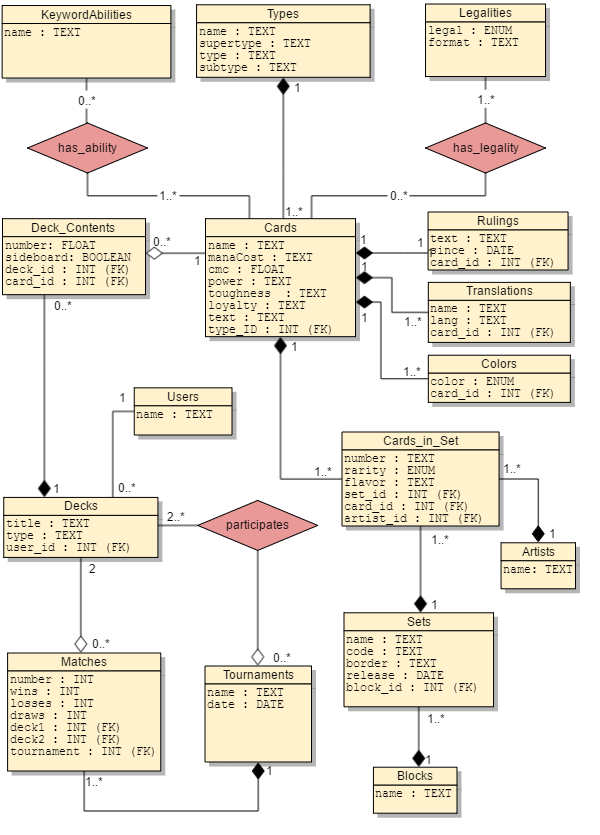
\includegraphics[width=\textwidth]{gfx/erm.png}
    \caption{Schema für relationale Datenbank}
    \label{fig:uml:schema}
\end{figure}

\begin{figure}[H]
    \myfloatalign
    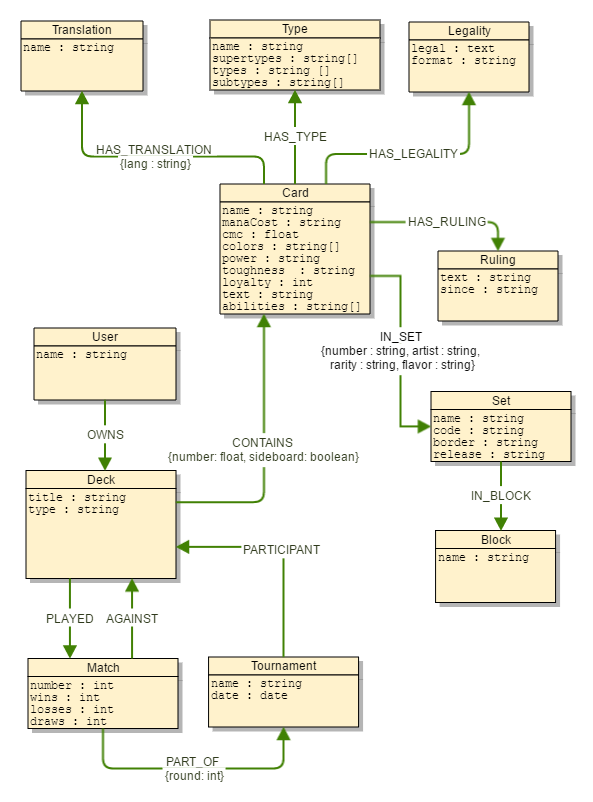
\includegraphics[width=\textwidth]{gfx/graph.png}
    \caption{Schema für Graph-Datenbank}
    \label{fig:graph:schema}
\end{figure}

\subsection{Beschreibung der Software-Komponenten}
%%%%%%%%%%%%%%%%%%%%%%%%%%%%%%%%%%%%%%%
%  * Dekomposition -> Softwarekomponenten + Beschreibung der Schnittstellen (Komponenten-Diagramm, siehe "SW-Architektur Webserver")
%  * Schnittstellenbeschreibung -> API für jedes Modul Model + Tabelle + Description (Klassen-Diagramm)
%%%%%%%%%%%%%%%%%%%%%%%%%%%%%%%%%%%%%%%

\begin{figure}[H]
    \myfloatalign
    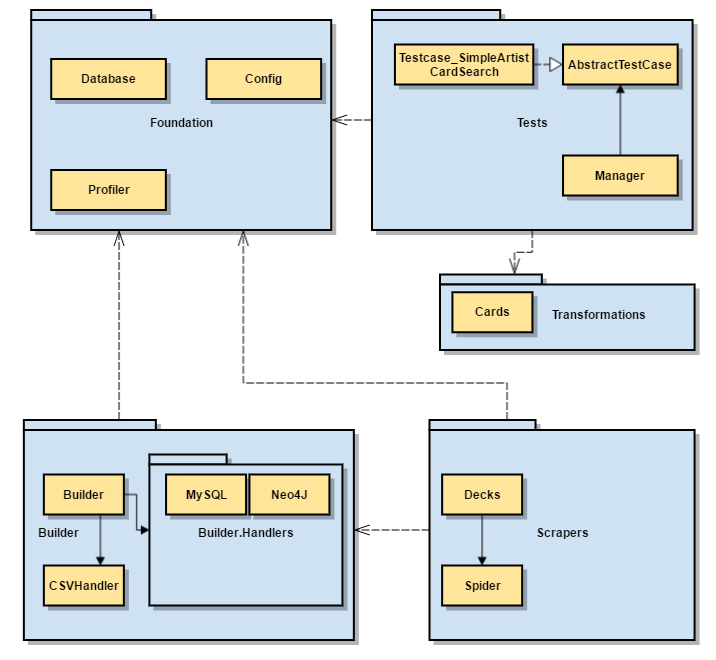
\includegraphics[width=\textwidth]{gfx/sw-components.png}
    \caption{Software-Komponenten}
    \label{fig:sw-components}
\end{figure}
\begin{description}
    \item[Builder] \hfill \\
        Das Package Builder ist zuständig für das erstellen und befüllen der Datenbanken.
    
    \item[Builder.Handlers]  \hfill \\
        Das Package Builder.Handlers enthält die Implementierungen für die konkreten Datenbanken
    
    \item[Scrapers]  \hfill \\
         Das Package Scrapers lädt Decks von mtgtop8 \footnote{mtgtop8 - http://mtgtop8.com/} herunter, um einen Datensatz für Decks und Turniere zu erstellen
    
    \item[Tests]  \hfill \\
        Enthält die konkreten Testfälle
    
    \item[Transformers]  \hfill \\
        Das Package Transformers ist zuständig für das Transformieren von Daten in eine vorgegebene Datenstruktur.
\end{description}

\subsection{Beschreibung der Schnittstellen}
%%% Beschreibung der Packet Schnittstellen. Scraper.Decks nutzt Spider um ..., Scraper.Decks nutzt Config? um ..
%%% evtl als liste ala:
%%% Scraper.Decks nutzt die folgenden Schnittstellen:
%%%   * Spider: Wird genutzt um webpage inhalt zu erhalten
%%%   * Foundation.Config: wird genutzt um xy zu erhalten
%%%   * ...
\subsubsection*{Builder}
Die Komponente \verb|Builder| nutzt die folgenden Schnittstellen:
\begin{description}
    \item[Foundation] wird genutzt um ein Datenbank-Verbindungen zu erstellen
\end{description}

\subsubsection*{Scrapers}
Die Komponente \verb|Scrapers| nutzt die folgenden Schnittstellen:
\begin{description}
    \item[Foundation] wird genutzt um auf die Konfiguration zuzugreifen
    
    \item[Builder] wird genutzt um die Decks in \ac{CSV} Dateien zu speichern
\end{description}

\subsubsection*{Tests}
Die Komponente \verb|Tests| nutzt die folgenden Schnittstellen:
\begin{description}
    \item[Foundation] wird genutzt um ein Datenbank-Verbindungen zu erstellen und mit dem \verb|Profiler| die Testfälle zu überwachen
    
    \item[Transformations] um die ausgelesenen Daten in eine passende Datenstruktur zu überführen
\end{description}
